\section{Introduction}

\subsection{Literature Review}
\begin{figure}[H]
    \centering
    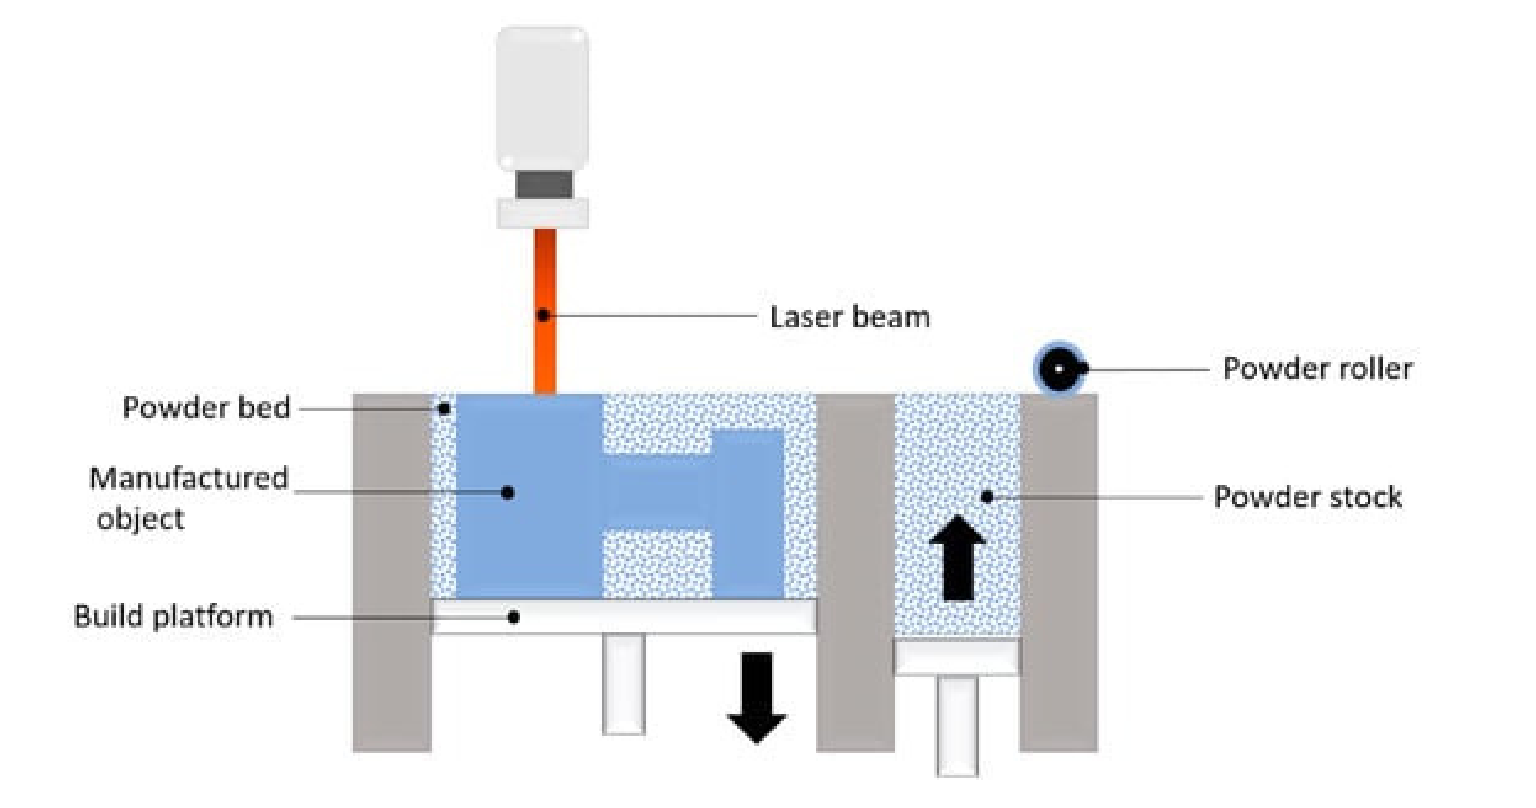
\includegraphics[width=5in]{Figures/Introduction/LPBF Overview.png}
    \caption[Schematic of LPBF]{Schematic of LPBF, from \cite{tebianian2023review}}
    \label{fig:LPBF Schematic}
\end{figure}
\begin{figure}[H]
    \centering
    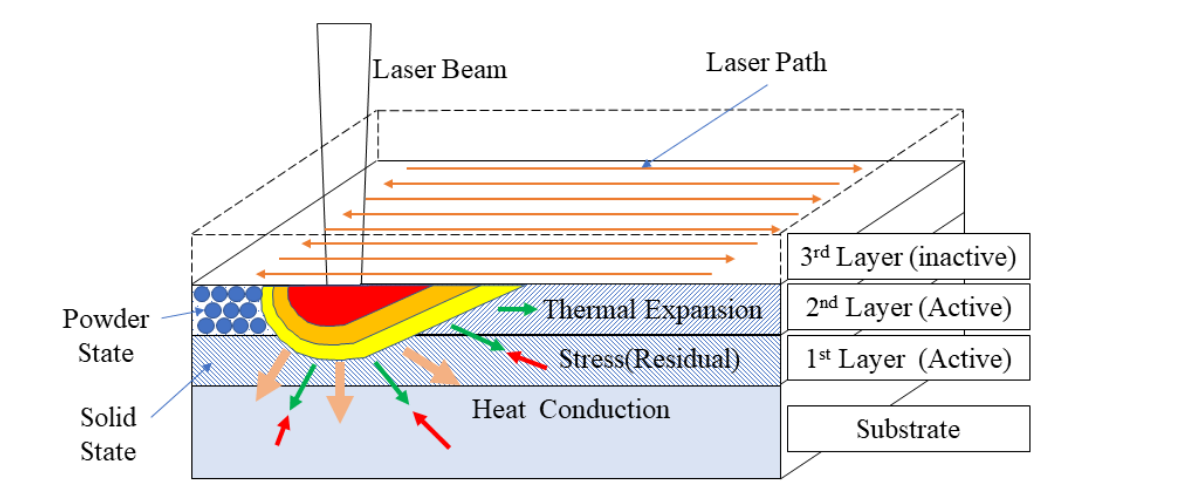
\includegraphics[width=5in]{Figures/Introduction/LPBF Section.png}
    \caption[Schematic heat and its effects on stress during LBPF ]{Schematic heat and its effects on stress during LPBF, from \cite{jung2022numerical}}
    \label{fig:LPBF Section}
\end{figure}
When printing a part, through powder bed fusion (see Figure \ref{fig:LPBF Schematic}) the laser traces a path around the bed of powder before new powder is added on top to start the next layer.  However, when heating the powder, the laser does not heat evenly; the center of the beam is narrow, but a wider area than just the beam is heated, but to a lower temperature than the center of the beam \cite{tebianian2023review}, \cite{deleon2025review}.  This difference in temperature means that different parts of the part will solidify at different times, and the differences in thermal expansion through this delta in effect stretches the part before it’s even complete.  This causes residual stress (see Figure \ref{fig:LPBF Section}).  The cold parts of the metal constrain the warm parts from cooling to a natural shape, pulling it in unwanted directions \cite{cai2024closed}.
The three parts of this literature review are: Residual Stresses in Powder Bed Fusion, How Print Orientation Affects Stress, and Simulation of Metal AM.  This was decided to cover the topic of residual stress, the factors that affect it, and how to simulate these stresses.
\subsection{Residual Stresses in Powder Bed Fusion}
Investigations into the stresses present in metal 3d printed parts have yielded valuable information.  Fojtik et al. \cite{fojtik2023quantification}, investigated the stresses present in a 3d printed brake pedal.  The most visible test of the stress was when they cut a part of the pedal.  The split piece opened up outwards like a flower, indicating that was the position it desired to be in; the state of lowest stress.  They also concluded that support materials produce additional residual stress in the areas immediately around them, due to the constant heat cycling that building the support creates, and the support’s role in locking the part into shape, rather than letting it expand and contract naturally. 

\begin{figure}[H]
    \centering
    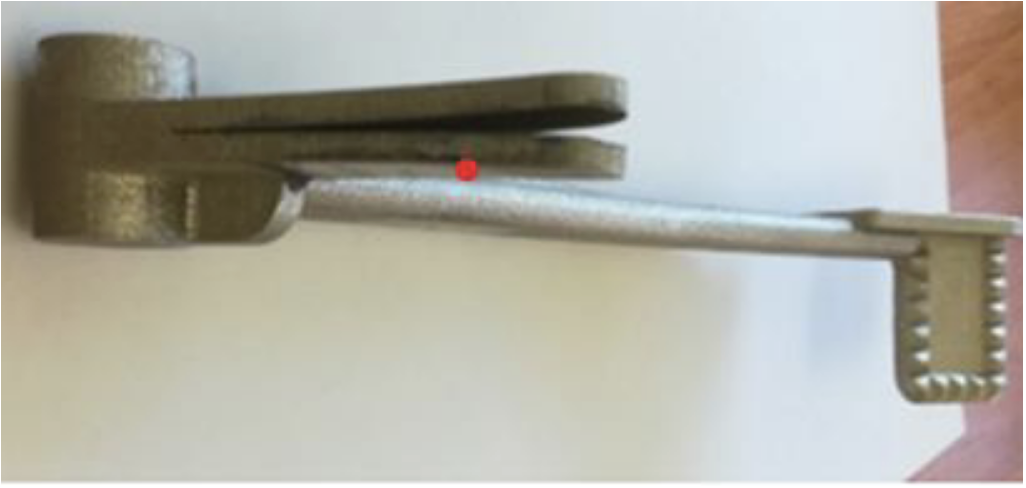
\includegraphics[width=3in]{Figures/Introduction/Brake Pedal.png}
    \caption[Deformation of a pedal printed by LPBF as a result of residual stresses]{Deformation of a pedal printed by LPBF as a result of residual stresses, from \cite{fojtik2023quantification}}
    \label{fig:Brake Pedal}
\end{figure}

An interesting finding from Park et al., was that the residual stresses on the last surface to be printed are tensile.  The mechanic behind this is;  the lower layers cool and shrink, but the top layer gets stuck on the layer below.  The molten metal bonds to the solid layer below, but when it contracts while solidifying, it is unable to contract as it naturally would \cite{park2024microstructure}.  However, once heat treated, the surface changed to compressive stress \cite{park2024microstructure}.  Depending on the application, this can be highly desirable, akin to shot peening in use.

\begin{figure}[H]
    \centering
    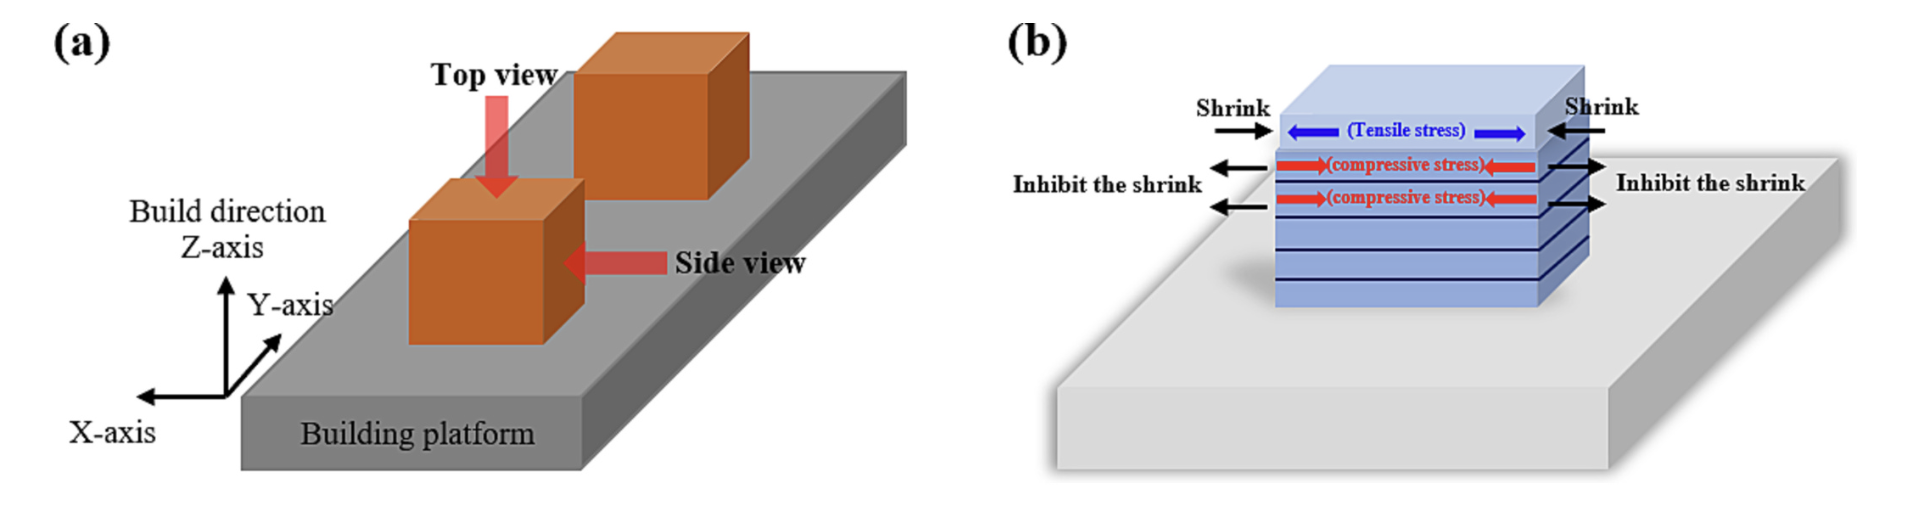
\includegraphics[width=5in]{Figures/Introduction/Stress causing shrinkage.png}
    \caption[Illustration of the stress-causing shrinkage]{Illustration of the stress-causing shrinkage, from \cite{park2024microstructure}}
    \label{fig:Shrinkage}
\end{figure}

\subsection{How Print Orientation Affects Stress}
One of the methods that is under study to remedy the problems of residual stress in a 3D print is to change the orientation of the prints.  
Yang et al. \cite{yang2024effect}, studied the effects of differing print orientations for parts printed via powder bed fusion. This group focused on the anisotropic effects of printing in layers with metal.  Their experiments yielded results akin to the anisotropy in a traditional FDM part.  The print layers are not as well bonded together as opposed to the metal made in one layer.  On the topic of building layers, Fojtik et al., studied the hatch pattern between layers and found that changing the raster pattern by 45 degrees between print layers reduces residual stress \cite{jung2022numerical}.  Takazawa et al. \cite{takezawa2022simultaneous}, studied the methods to reduce warpage in a printed part by manipulating the orientation of the hatches and the infill density.  By optimizing these two parameters, part warpage is decreased, inferring that there is a reduction in residual stress as well; as the part does not bend on its own \cite{takezawa2022simultaneous}.  

\subsection{Simulation of Metal AM}
Simulation of parts made via 3D printing can be accomplished using softwares like ANSYS.  Alzyod and Ficzere \cite{alzyod2023material}, \cite{alzyod2023rapid} experimented with the simulation techniques available in traditional 3d printers in two papers (FDM, SLA, etc.).  They found that the residual stresses can be accurately predicted using simulation combined with empirical data.  In their study, they ran simulations, printed parts, tested them, and went back and tuned the simulation based on the stresses in the real parts.  This allows for accurate simulation of more complex parts based on the simulations that have been tuned.  Zelder et al. \cite{zelder2025learning} trained a PointNet architecture to optimize part orientation for printing by LPBF.  This work is optimized for cost, geometric accuracy, and print time.  Residual stress was mentioned, but not explored as one of the variables in the process.  Their parts were rotated in space, attempting to minimize support structures, z-height (which increases time) and keep geometric stability (like errors based on layers  in the AM process) \cite{zelder2025learning}.  
\subsubsection{ANSYS Analysis}
\indent Weinhold et al. \cite{weinhold2021simulation} ran a manual version of this optimization problem for their conference paper.  To take advantage of the 3D printing process, they used topology optimization to find the minimum amount of material needed to build a functional connecting rod for a 212cc engine.  Then, they ran simulations at three orientations: 0, 45, and 90 degrees to find which had the least distortion.  Their paper found that 0 degrees of rotation (horizontal) had the least distortion (and by extension residual stress) \cite{weinhold2021simulation}.
\begin{figure}[H]
    \centering
    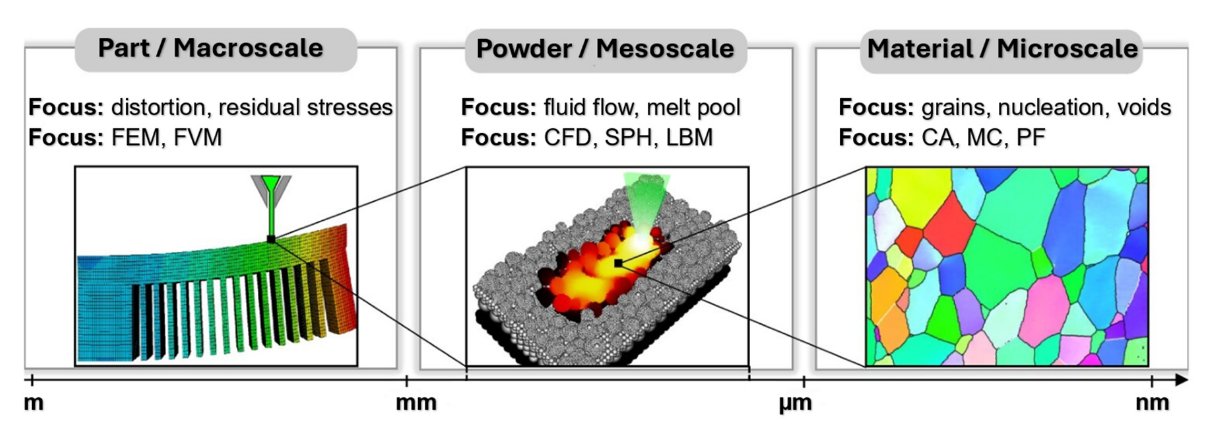
\includegraphics[width=5in]{Figures/Introduction/LPBF Scales.png}
    \caption[The three scales of LPBF simulation]{The three scales of LPBF simulation, from \cite{kascak2025review}}
    \label{fig:simscales}
\end{figure}
\indent Kaskac et al. \cite{kascak2025review} describe the different types of LPBF analysis in their paper, as shown in Figure \ref{fig:simscales}.  Microscale focuses on heating, voids, etc. at the grain structure level.  Mesoscale looks at the scale of the melt pool (0.01-1.0mm) and macroscale looks at the part level.  This report focuses on the macroscale, as does ANSYS.
\newline \indent Kaskac et al. \cite{kascak2025review} makes some notes about the ANSYS method of simulation in their paper.  ANSYS simulates each individual voxel layer in the mesh as one scan layer, and there are three levels of simulation for LPBF: assumed uniform stress, scan pattern, and thermal stress (thermal stress will be used for this paper).  They also note that ANSYS does not always take into account the moving heat source when the dominant thermal gradient is in the opposite direction \cite{kascak2025review}.

\subsubsection{Analysis of Other AM Methods}
\indent Another method of manufacturing metal parts is through direct energy deposition.  Rong et al. \cite{rong2024thermal} have done work in predicting the residual stresses associated with this method of manufacture through FEA.  To accurately model the material that is produced from melting through cooling, the different phases through which a material (steel) will pass through are added to the FEA model \cite{rong2024thermal}.  While cooling, phases such as martensite and bainite are formed, and they each have different rates of cooling, thermal expansion, etc.  So incorporating the different possible phases into the model will increase its accuracy over just having a single phase being cooled \cite{rong2024thermal}.  The process of direct energy deposition is different from LPBF, however, the principles that create the residual stress are the same.
\subsection{Status and Outlook}
The field of residual stresses in powder bed fusion prints is one undergoing a plentiful research.  It seems that the underlying causes are reasonably well understood.  Lab work specifically in reducing the residual stress seems somewhat lacking, however.  As shown in the paper by Park et al. \cite{park2024microstructure}, having broad, flat surfaces normal to the direction of printing bed travel causes high residual stress buildups.  One avenue to explore would be diagonalizing the print to reduce this stress.  At a minimum, this would reduce the tensile stress lengthwise along the top print surface, however, this would cause new stress patterns to show up in the cross section of the part.  
\newline \indent Work has been done using deep learning to optimize part print orientation, but without concerning residual stresses.  These different research instances can be used together to optimize for the residual stress and print orientation problem.  The pattern of laser travel has also been studied, but it doesn’t seem like part orientation in space has garnered much attention yet.  An investigation into the orientation of prints within 3D space will complement the work that has already been done into surface stresses and raster orientation in prints.
